\documentclass[../main.tex]{subfiles}

\begin{document}
\section{Results}\label{sec:results}
\subsection{Franke's function}
\subsubsection{Actual prediction of data}
We use a dataset of $N=100$ datapoints generated from the Franke function (including noise from the normal distribution, with $\sigma=0.1$), and split it into a training and testing set. Figure \ref{fig:result_actual_plot} shows the testing set plotted in 3D, which is what we aim at recreating.

\begin{figure}[h]
    \centering
    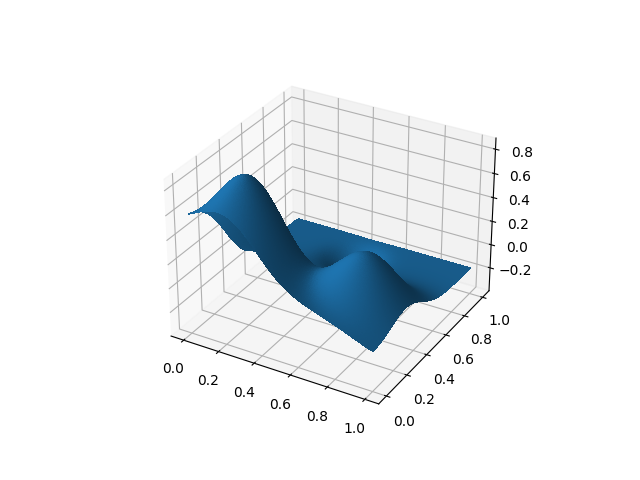
\includegraphics[width=\textwidth]{../assets/actual_franke_plot.png}
    \caption{Real valued plot of the testing set of a dataset generated from the Franke function.}
    \label{fig:result_actual_plot}
\end{figure}

Figure \ref{fig:result_reg_plots} shows the predictions of this data, using different regression methods. There's some apparent overfitting in the OLS regressed model. The Ridge model comes quite close, while the Lasso does not give any satisfactory results. 

\begin{figure}[htb!]
    \centering
    \begin{subfigure}[b]{0.48\textwidth}
        \centering
        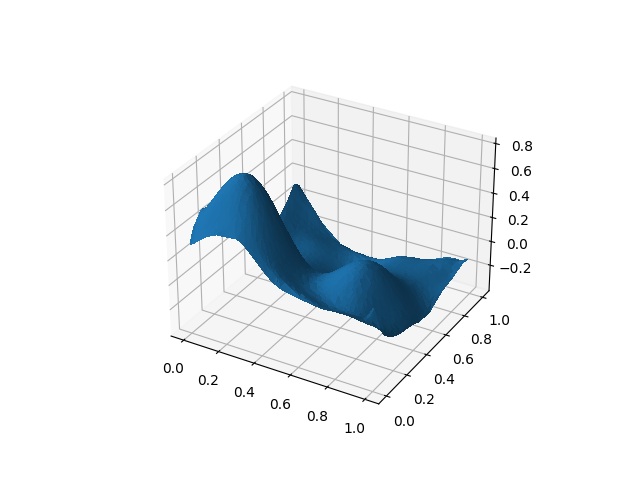
\includegraphics[trim=2.4cm 1cm 1.4cm 1cm, clip,width=1.1\textwidth]{../assets/ols_franke_plot.png}
        \caption{OLS}
        \label{fig:result_ols_plot}
    \end{subfigure}
    \quad
    \begin{subfigure}[b]{0.48\textwidth}
        \centering
        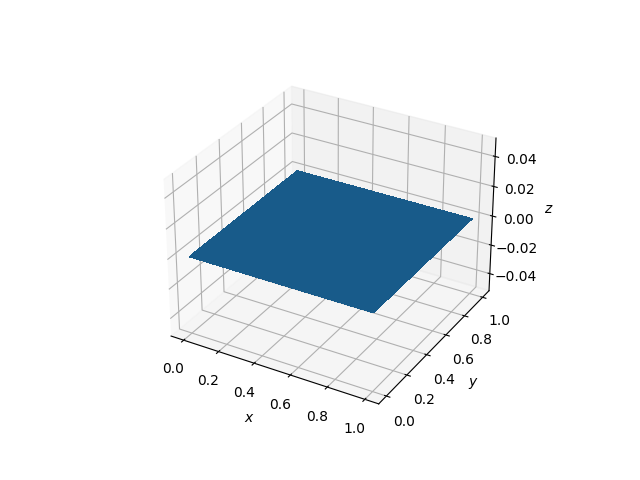
\includegraphics[trim=2.4cm 1cm 1.4cm 1cm, clip,width=1.1\textwidth]{../assets/lasso_franke_plot.png}
        \caption{Lasso}
    \end{subfigure}
    
    \begin{subfigure}[b]{0.48\textwidth}
        \centering
        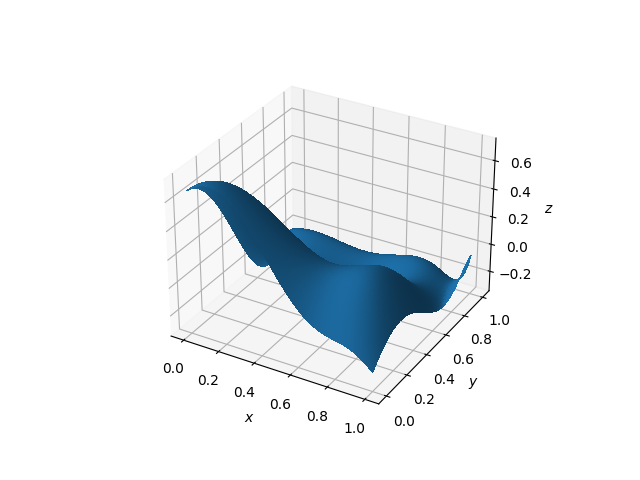
\includegraphics[trim=2.4cm 1cm 1.4cm 1cm, clip,width=1.1\textwidth]{../assets/ridge_franke_plot.png}
        \caption{Ridge}
    \end{subfigure}
    \caption{Prediction of the data shown in figure \ref{fig:result_actual_plot} using different regression methods.}
    \label{fig:result_reg_plots}
\end{figure}

The confidence intervals was also calculated and can be seen in figure \ref{fig:OLS_CI_franke}.

\begin{figure}[H]
 \centering
    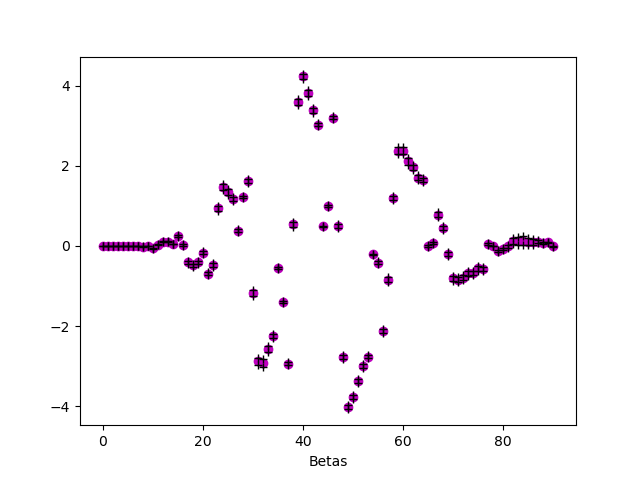
\includegraphics[width=0.8\textwidth]{../assets/ols_franke_CI.png} 
    \caption{The regression parameters $\beta$ for the OLS regression method, calculated with a confidence interval of 95\%}
    \label{fig:OLS_CI_franke}
\end{figure}


\subsubsection{The bias-variance tradeoff}
With a dataset of values produced from Franke's function (number of datapoints $N=18$, with random normally distributed noise added), we've fitted a model based on the training set and predicted new data based on the testing set. This was done with a design matrix of increasing degrees, from $1$ to $9$. The following figure \ref{fig:result_complexity} is a plot relating the mean squared error of the model to the complexity (or degree).

\begin{figure}[h]
    \centering
    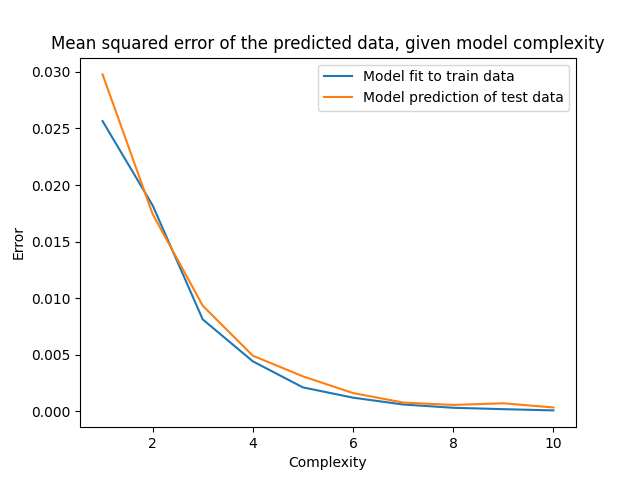
\includegraphics[width=\textwidth]{../assets/complexity.png}
    \caption{The error of a model based on the train and test set respectively, in relation to the polynomial degree of the model.}
    \label{fig:result_complexity}
\end{figure}

Once again, we produce a dataset from the Franke function (number of datapoints $N=40$, no noise added) and fit the model to design matrices of varying degree, from 1 to 15. Using The Bootstrap, we record the bias and variance (as they are explained in section \ref{sec:bv_decomp}. Figure \ref{fig:result_bias_variance} shows their relation with increasing complexity/degree of polynomial. 

\begin{figure}[h]
    \centering
    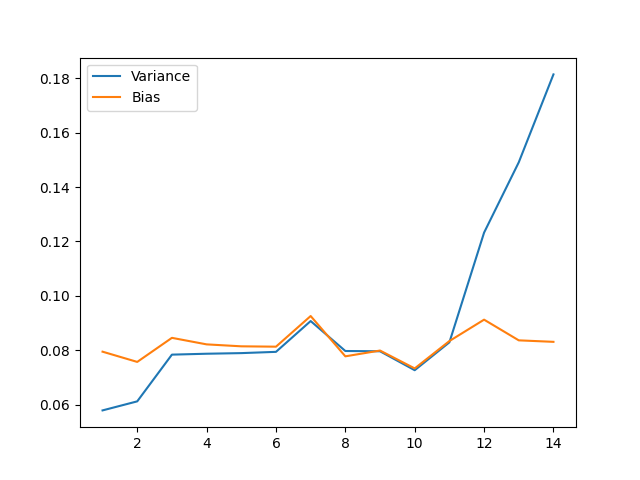
\includegraphics[width=\textwidth]{../assets/var.png}
    \caption{Bias and variance plotted in relation to the polynomial degree of the model.}
    \label{fig:result_bias_variance}
\end{figure}

The above results uses bootstrapping as an assessment technique. We have also implemented $K$-fold cross-validation, and figure \ref{fig:result_cv_boot_mse} shows how their calculated MSE compares

\begin{figure}[h]
    \centering
    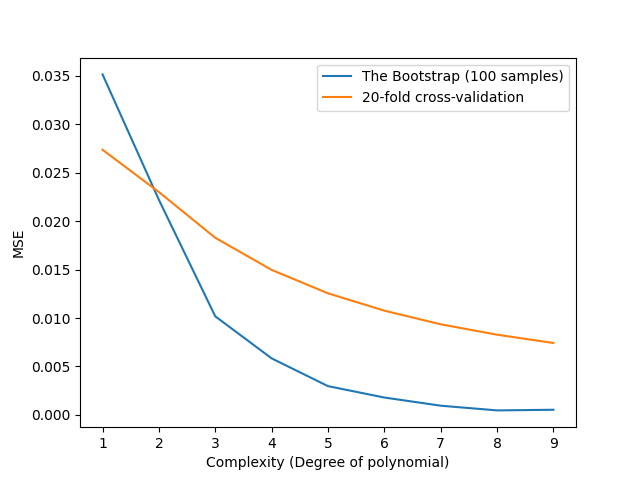
\includegraphics[width=\textwidth]{../assets/cv_boot_mse.png}
    \caption{Mean squared error calculated with $K=20$-fold cross-validation and bootstrapping with $B=100$.}
    \label{fig:result_cv_boot_mse}
\end{figure}

\subsection{Terrain data}
The models were tested on terraindata over Norway. The full terrain that the project was based on can be seen in figure \ref{fig:terrain_Norway}. The small patch from the terrain data that was analyzed by using the regression models can be seen in figure \ref{fig:terrain_Norway_patch}. The size of the patch analyzed was 20 datapoints in each direction, making a total of 400 datapoints.

\begin{figure}[H] 
   \centering
   \begin{subfigure}[b]{0.35\textwidth}
    \centering
    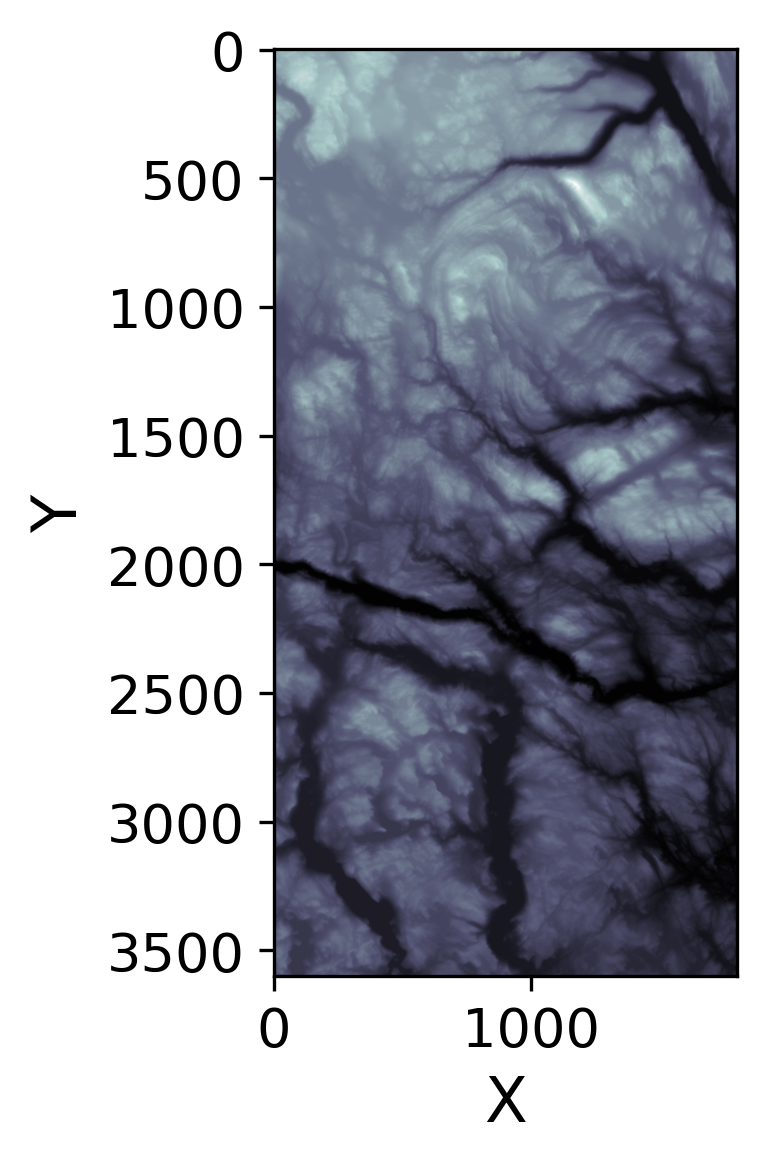
\includegraphics[width=\textwidth]{../assets/Terrain_SRTM_data_norway_1.png} 
    \caption{}
    \label{fig:terrain_Norway}
   \end{subfigure}
   \quad
   \begin{subfigure}[b]{0.55\textwidth}
    \centering
    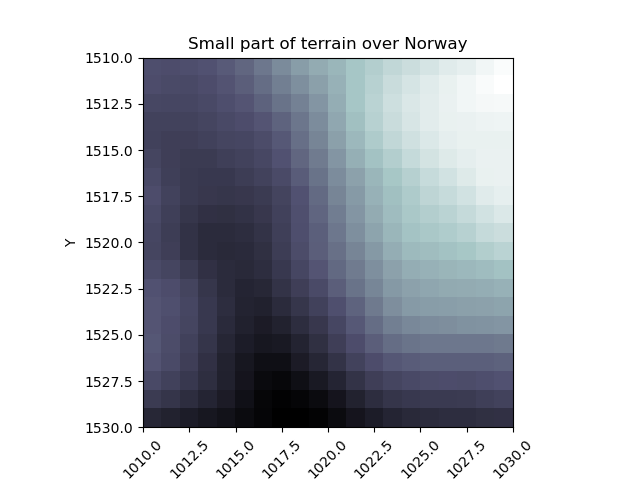
\includegraphics[width=\textwidth]{../assets/part_of_terrain.png} 
    \caption{}
    \label{fig:terrain_Norway_patch}
   \end{subfigure}
   \caption{(a) Terrain data over Norway. (b) Small part of the terrain data consisting of 400 datapoints.}
\end{figure} 

\subsubsection{OLS}
Ordinary least squares method was performed on the terrain data, the results from  \autoref{fig:test-train-error} shows the test-train error-plot obtained by using cross validation with increasing degree to find the polynomial degree which gives the lowest MSE for linear regression. A minimum is reached at \ensuremath{d=12}. \autoref{fig:OLS-estimate} shows the result of performing OLS with $d=12$ on the terrain dataset. We obtain MSE and R2-scores of 160.9 and 0.9156, respectively. 


\begin{figure}[H] 
   \centering
   \begin{subfigure}[b]{0.51\textwidth}
      \centering
    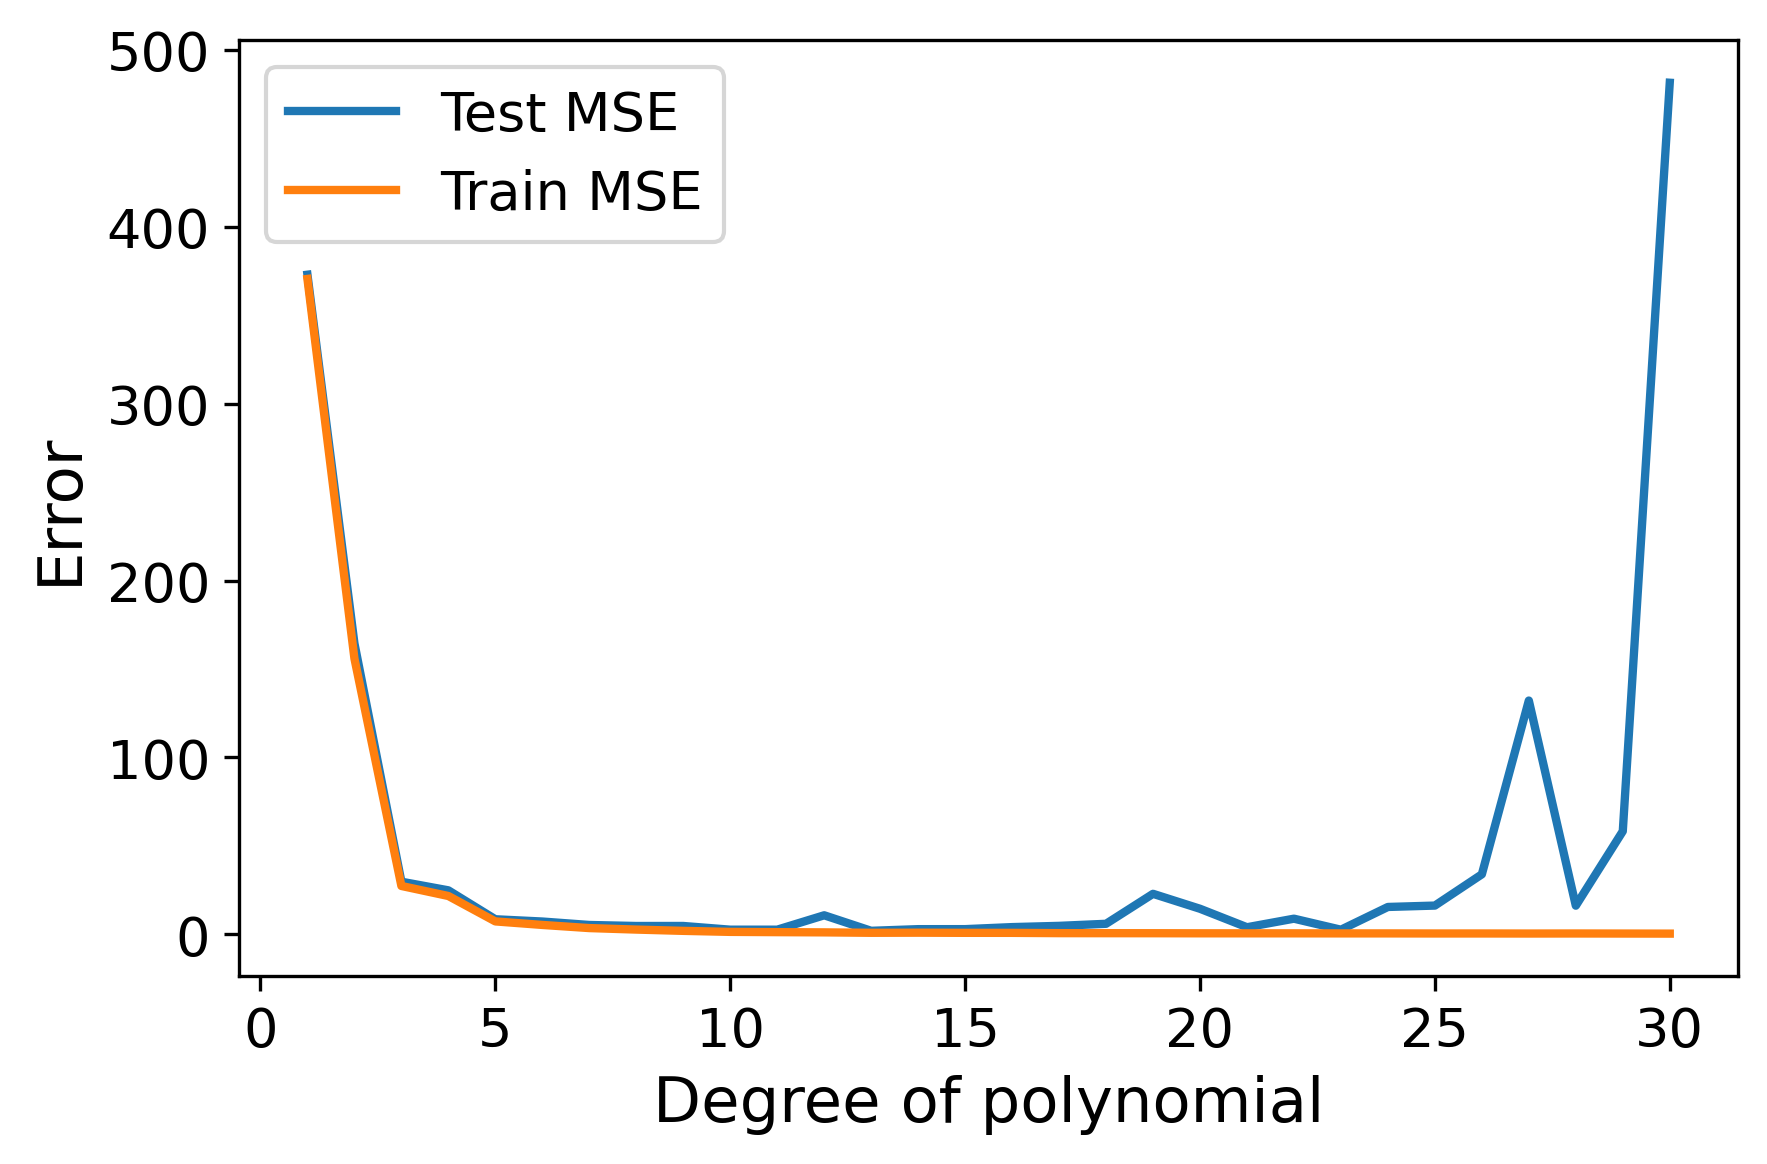
\includegraphics[width=\textwidth]{../assets/terrain_ols_error_plot.png}
    \caption{}
    \label{fig:test-train-error}
   \end{subfigure}
   \quad
   \begin{subfigure}[b]{0.45\textwidth}
    \centering
    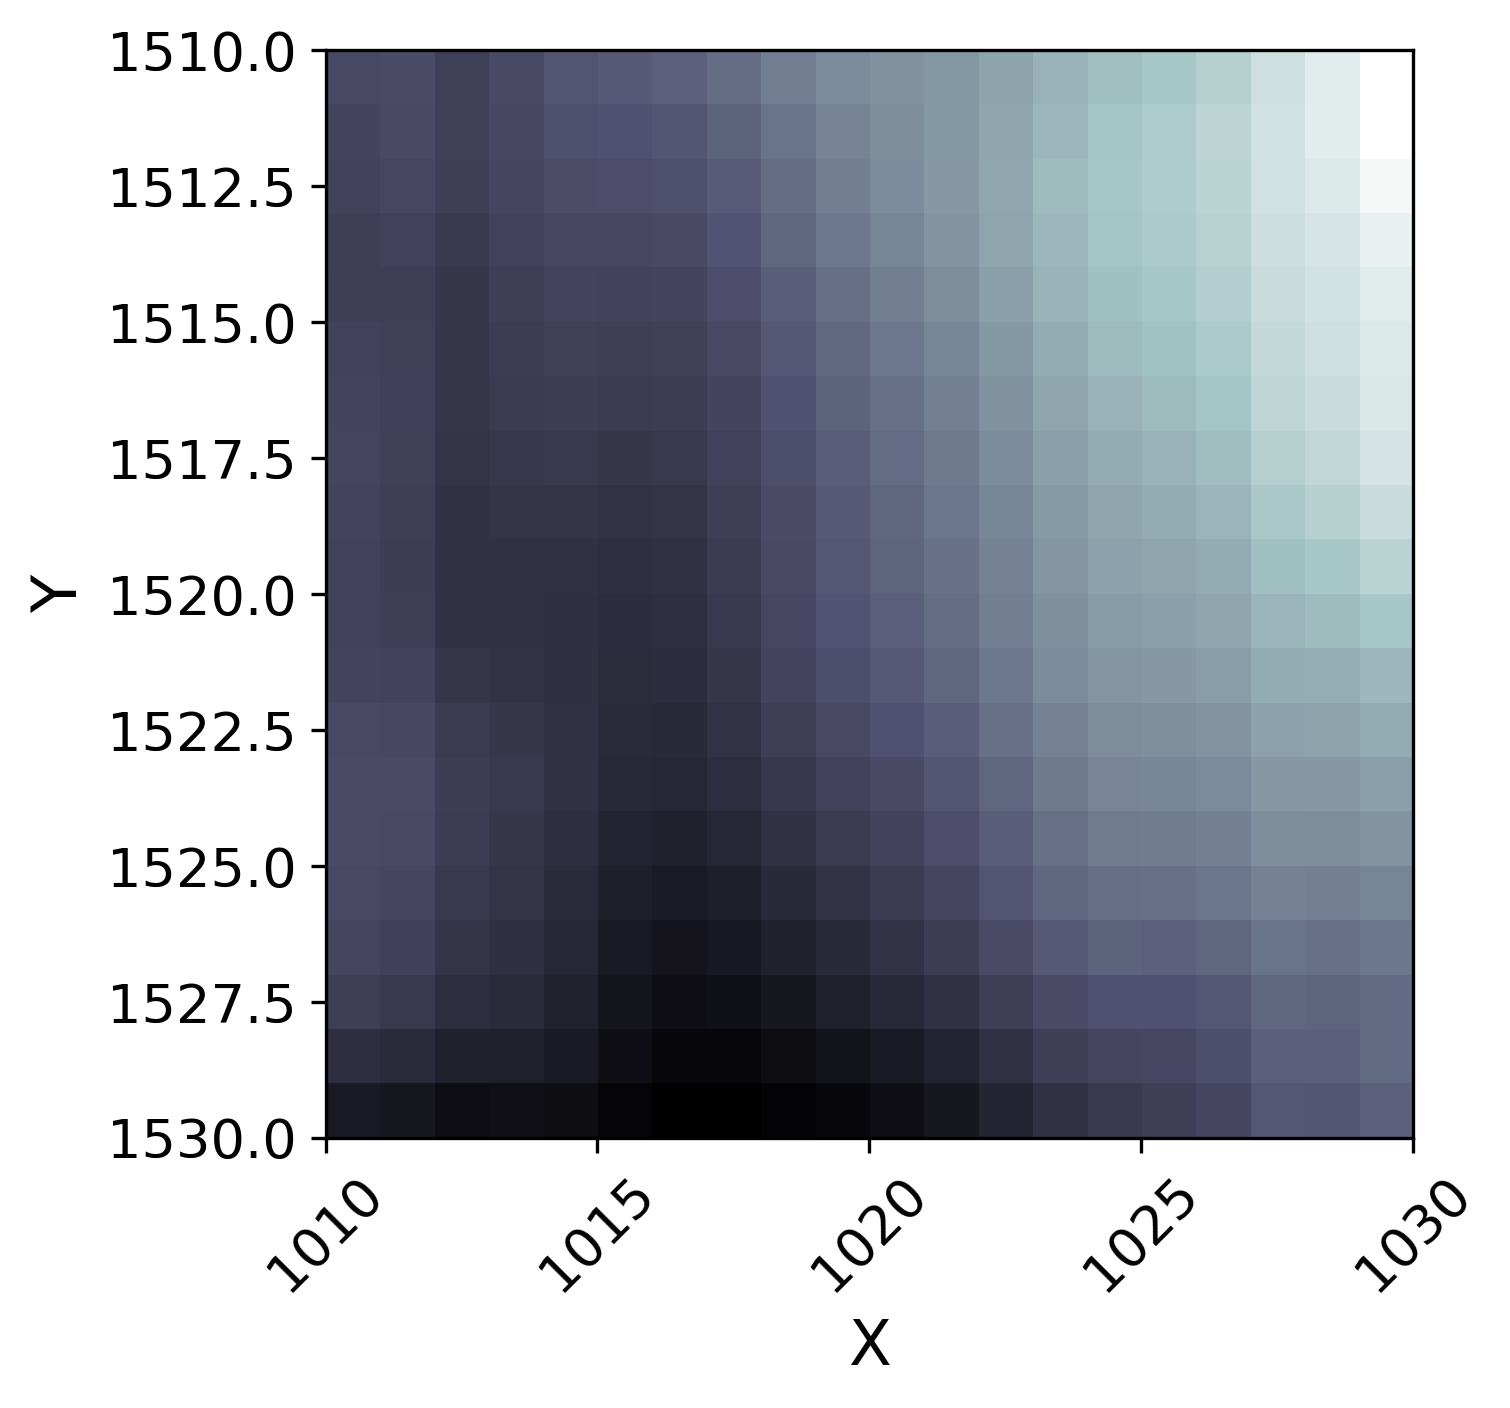
\includegraphics[width=\textwidth]{../assets/Terrain_OLS_bestdegree_newnew.png} 
    \caption{}
    \label{fig:OLS-estimate}
   \end{subfigure}
   \caption{(a) The test and training error as a function of polynomial degree. (b) The result of OLS performed on the terrain data with degree=12
   }
   \label{fig:terrain-OLS}
\end{figure} 

The confidence intervals of the parameters $\beta$ were also calculated for the OLS regression. The regression parameters $\beta$ are shown in figure \ref{fig:OLS_CI}.

\begin{figure}[H]
 \centering
    \includegraphics[width=0.8\textwidth]{../assets/terrain_OLS_CI_new.png} 
    \caption{The regression parameters $\beta$ for the OLS regression method, calculated with a confidence interval of 95\%}
    \label{fig:OLS_CI}
\end{figure}


\subsubsection{Ridge regression}
\autoref{fig:ridge_regularization} depicts the computed regularization path MSE$(d,\log_{10}(\lambda))$ with 5-fold cross validation. The minimum MSE is found to be 2.020 for \ensuremath{d=19} and \ensuremath{\lambda=1.311\cdot 10^{-10}}. \autoref{fig:ridge_estimate} shows the result of performing Ridge regression with $d=19$ and $\lambda=1.311\cdot 10^{-10}$ on the terrain dataset. We obtain MSE and R2-scores of 0.9099 and 0.9995, respectively. 

\begin{figure}[H] 
   \centering
   \begin{subfigure}[b]{0.56\textwidth}
    \centering
    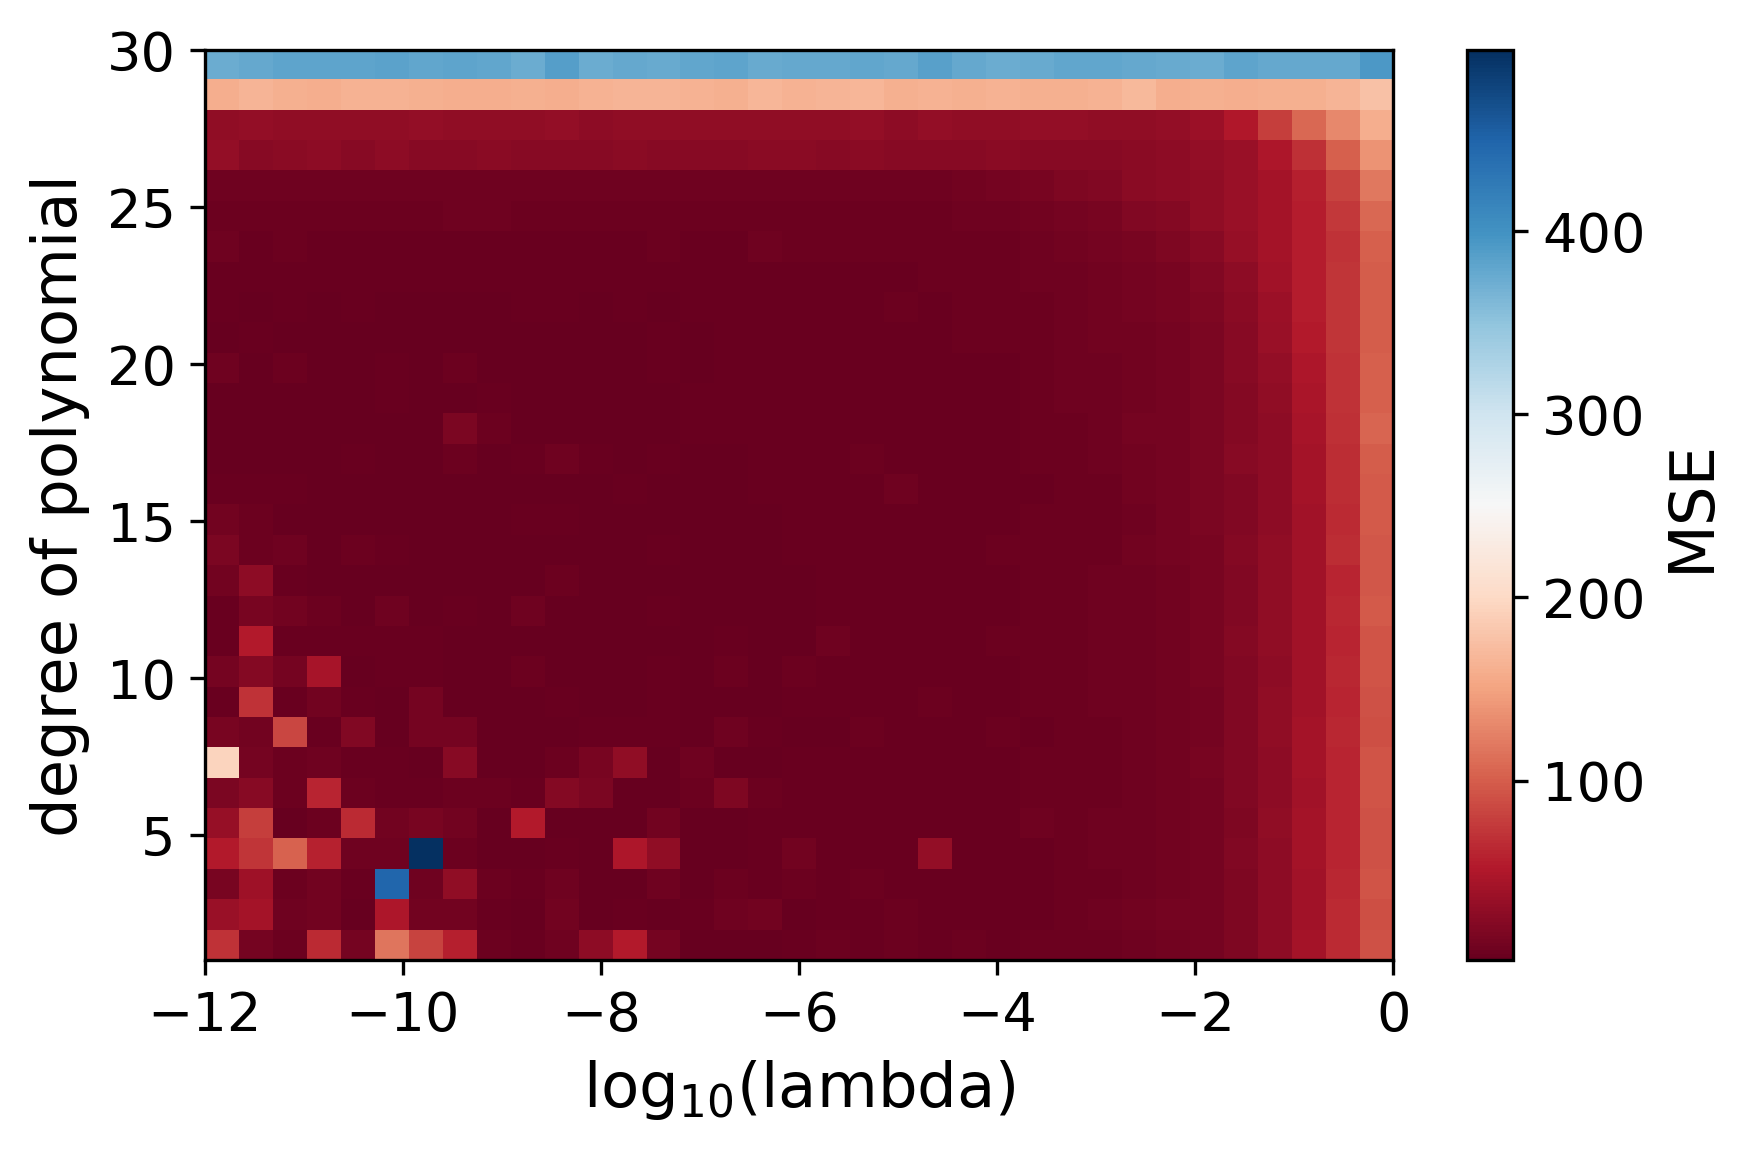
\includegraphics[width=\textwidth]{../assets/terrain-ridge-degree-lambda-colormap.png} 
    \caption{}
    \label{fig:ridge_regularization}
   \end{subfigure}
   \quad
   \begin{subfigure}[b]{0.4\textwidth}
    \centering
    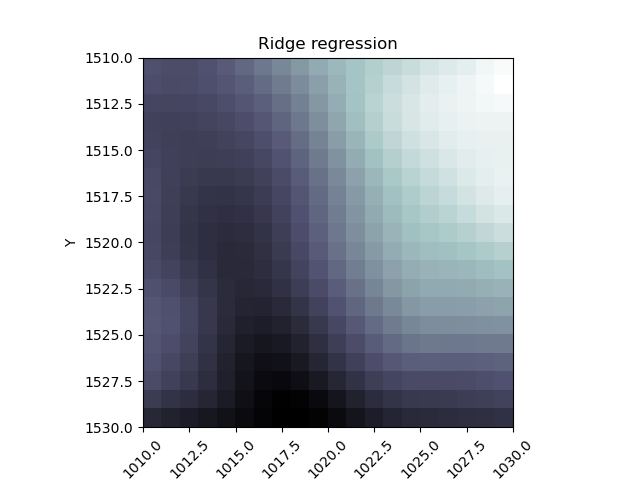
\includegraphics[width=\textwidth]{../assets/Terrain_ridge_bestdegree.png} 
    \caption{}
    \label{fig:ridge_estimate}
   \end{subfigure}
   \caption{(a) Color map: Defining the MSE by color. The MSE is calculated for every combination of $\lambda$ and the degree of polynomial. Degrees up to 30 and $\lambda$ in the interval $\log_{10}[ -12,0 $] divided into 35 uniformly spaced values, was used to find the best parameters. \\ (b) The result of Ridge performed on the terrain data with degree=19 and $\lambda=1.311\cdot 10^{-10}$.
   }
   \label{fig:terrain-ridge}
\end{figure} 

Ridge method was also performed with smaller spacing of $\lambda$ in a smaller interval. Letting $\lambda$ iterate in the interval $\log_{10}[ -4,0 $] with the minimum MSE found to be 5.043 for \ensuremath{d=22} and \ensuremath{\lambda=0.0001\cdot 10^{-10}}. The obtained MSE and R2-scores are 3.748 and 0.9980, respectively. The colormap and the terrain for this run can be seen in the github folder under \verb|terrain_result/OLS_terrain|. 

\subsubsection{Lasso regression}
\autoref{fig:lasso_regularization} depicts the computed regularization path MSE$(d,\log_{10}(\lambda))$ with 5-fold cross validation. The minimum MSE is found with \ensuremath{d=21} and \ensuremath{\lambda=1.51 \cdot 10^{-3}}. \autoref{fig:lasso-estimate} shows the result of performing Ridge regression with $d=121$ and $\lambda=1.51 \cdot 10^{-3}$ on the terrain dataset. We obtain MSE and R2-scores of 9.56 and 0.9949, respectively.

\begin{figure}[H] 
   \centering
   \begin{subfigure}[b]{0.56\textwidth}
    \centering
    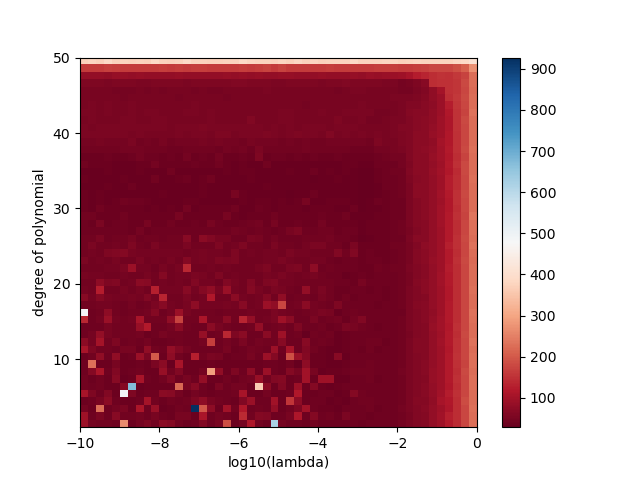
\includegraphics[width=\textwidth]{../assets/terrain-lasso-degree-lambda-colormap.png} 
    \caption{}
    \label{fig:lasso_regularization}
   \end{subfigure}
   \quad
   \begin{subfigure}[b]{0.4\textwidth}
    \centering
    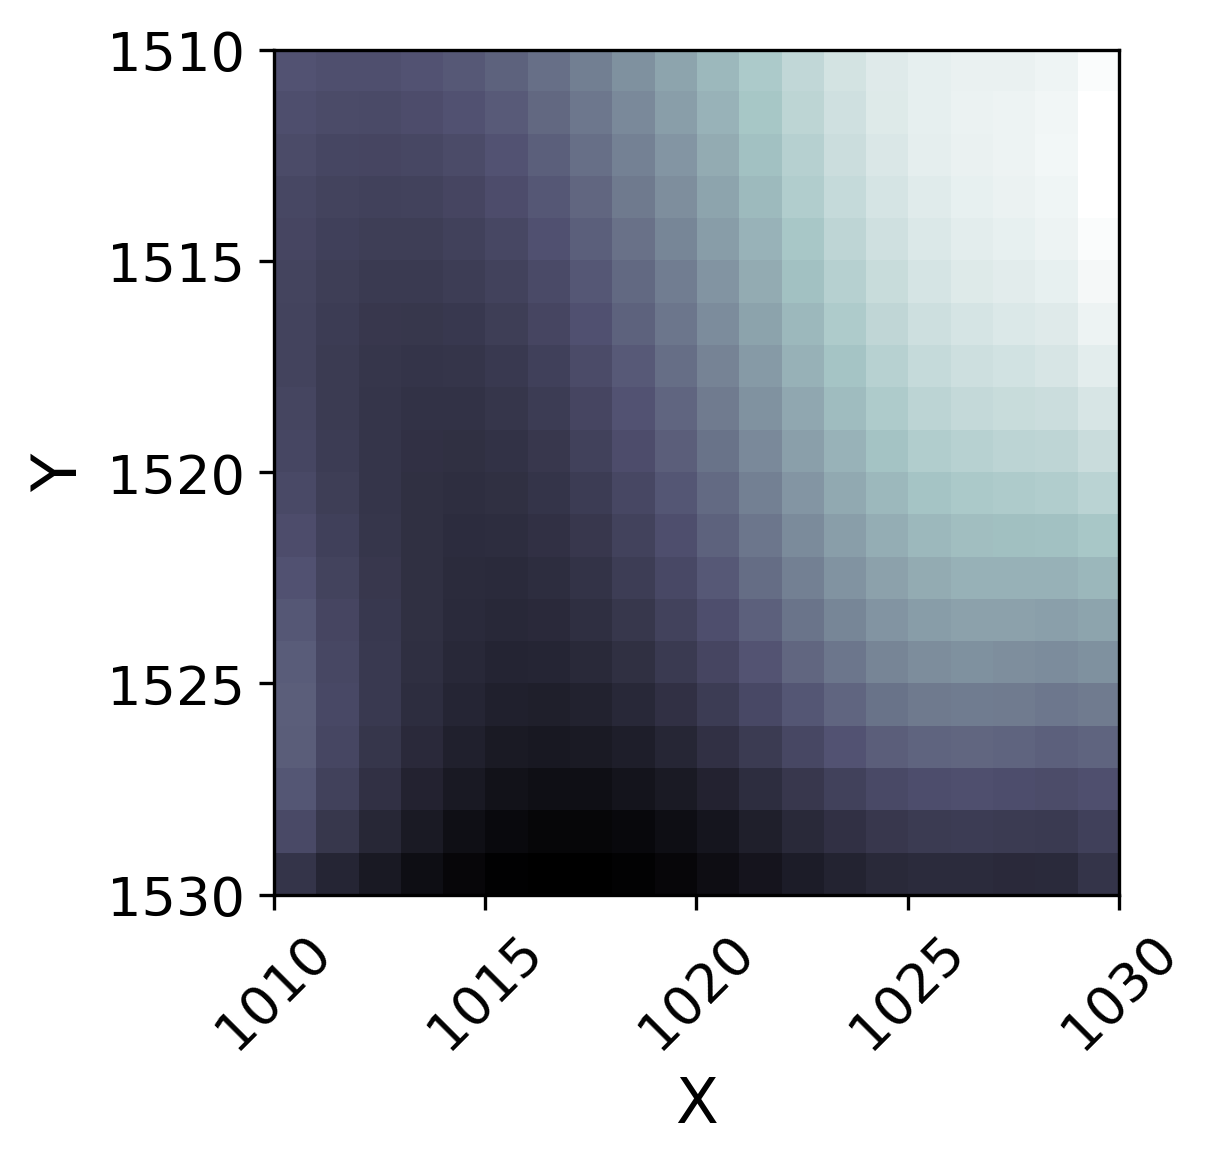
\includegraphics[width=\textwidth]{../assets/Terrain_lasso_bestdegree.png} 
    \caption{}
    \label{fig:lasso-estimate}
   \end{subfigure}
   \caption{(a) Color map: Defining the MSE by color. The MSE is calculated for every combination of $\lambda$ and the degree of polynomial. Degrees up to 50 and $\lambda$ in the interval $\log_{10}[ -12,0 $] divided into 50 uniformly spaced values was used to find the best parameters. \\ (b) The result of Lasso performed on the terrain data with degree=21 and $\lambda=1.51 \cdot 10^{-3}$.}
   \label{fig:terrain-lasso}
\end{figure} 

\end{document}
